\documentclass[tikz,border=10pt]{standalone}
\usetikzlibrary{intersections} % 加载交点库
\usepackage{mathrsfs}

\begin{document}
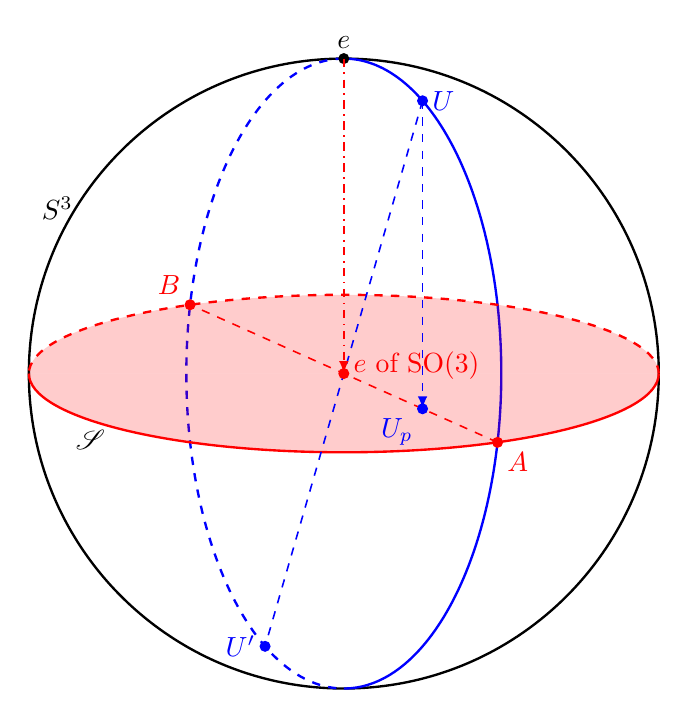
\begin{tikzpicture}
	% 绘制圆
	\draw[line width =0.3mm] (0,0) circle (4cm);
	\node at ({4.2cm* cos(150)},{4.2cm*sin(150)}) {$S^3$};
	% 绘制竖直椭圆
	\draw[line width=0.3mm, name path=ellipse1,blue] (0,-4cm) arc (-90:90:2cm and 4cm);
	\draw[line width = 0.3mm,dashed, name path = ellipse2,blue] (0,4cm) arc (90:270:2cm and 4cm);

	% 绘制水平椭圆
	\draw[fill,fill opacity = 0.2,line width = 0.3mm, name path=ellipse3,red] (-4cm,0) arc (-180:0:4cm and 1cm);
	\draw[fill,fill opacity = 0.2,line width = 0.3mm,dashed, name path =ellipse4,red] (4cm,0) arc (0:180:4cm and 1cm);
	\node at({4.2cm*cos(220)},{1.3cm * sin(220)}){$\mathscr{S}$};

	% 找到交点
	\path[name intersections={of=ellipse1 and ellipse3, by={A}}];
	\path[name intersections={of=ellipse2 and ellipse4, by={B}}];

	% 标记交点
	\fill[red] (A) circle (2pt) node[below right] {$A$};
	\fill[red] (B) circle (2pt) node[above left] {$B$};

	% 连接交点
	\draw[line width=0.2mm, dashed,red,name path = AB] (A) -- (B);

	\coordinate (U) at (60: 2cm and 4cm);
	\coordinate(U') at (240:2cm and 4cm);
	\fill[blue] (U) circle(2pt)node[right] {$U$};
	\fill[blue] (U') circle(2pt)node[left] {$U'$};
	\draw[line width = 0.2mm,dashed,blue] (U) -- (U');

	\fill[] (0,4cm) circle(2pt) node[above]{$e$};
	\fill[red] (0,0) circle(2pt) node[right,yshift = 1mm]{$e$ of SO(3)};
	\draw[line width = 0.2mm,dash dot,red,-latex] (0,4cm) -- (0,0);

	\path[name path = Uline](U) -- (-60:2cm and 4cm);
	\path[name intersections = {of = Uline and AB,by = {Uprojection}}];
	\fill[blue] (Uprojection) circle(2pt) node [below left]{$U_p$};
	\draw[blue,line width = 0.2mm , dashed , -latex] (U)--(Uprojection);


\end{tikzpicture}
\end{document}
